\documentclass[10pt]{memoir}

% based on kieran healy's memoir modifications
\usepackage{mako-mem}
\chapterstyle{article-3}
\pagestyle{memo}

\usepackage{ucs}
\usepackage[utf8x]{inputenc}

\usepackage[T1]{fontenc}
\usepackage{textcomp}
\usepackage[garamond]{mathdesign}

\usepackage[letterpaper,left=1.2in,right=1.2in,top=1.15in,bottom=1.1in]{geometry}

% packages i use in essentially every document
\usepackage{graphicx}
\usepackage{wrapfig}
\usepackage{enumerate}

% packages i use in many documents but leave off by default
% \usepackage{amsmath, amsthm, amssymb}
% \usepackage{dcolumn}
% \usepackage{endfloat}

% import and customize urls
\usepackage[usenames,dvipsnames]{color}
\usepackage[breaklinks]{hyperref}

\hypersetup{colorlinks=true, linkcolor=Black, citecolor=Black, filecolor=Blue,
    urlcolor=Blue, unicode=true}

% add bibliographic stuff 
% \usepackage[round]{natbib}
% \def\citepos#1{\citeauthor{#1}'s (\citeyear{#1})}
% \def\citespos#1{\citeauthor{#1}' (\citeyear{#1})}

% import vc stuff after running `make vc`: \input{vc} \pagestyle{kjhgit}

\begin{document}

\setlength{\parskip}{4.5pt}

\baselineskip 14.5pt

\title{Research Statement}
\author{Benjamin Mako Hill}

\maketitle

I study collective action in online communities and seek to understand
why some attempts at collaborative production -- like Wikipedia and
Linux -- build large volunteer communities while the vast majority
never attract even a second contributor. I am particularly interested
in how the design of communication and information technologies shape
fundemental social outcomes with broad theoretical and practical
implications -- like the decision to join a community or contribute to
a public good. My research is deeply interdisciplinary, consists
primarily of ``big data'' quantitative analyses, and lies at the
intersection of sociology, communication, and human-computer
interaction.

Using Internet-based peer production projects as my research settings,
my work seeks to understand the conditions for collective action using
observational data from real communities.  This work has been shaped
by three complentary approaches: (1) the comparison of failures to
build communities to rare successful attempts; (2) attention to the
role of reputation and status in the mobilization of volunteers; and
(3) analysis of design changes as ``natural experiments'' building a
deeper, and often causal, understanding from observational
data. Nearly all of my work incorporates at least two of these
approaches.

\section{Studying Attempts at Collective Action}

Although there have been many thousands of studies of online
collective action, the vast majority have only considered projects
like Wikipedia and Linux that have successfully built communities -- a
characterization that can be extended to observational work on
collective action more generally. In this sense, most previous
analyses have systematically selected on their dependent
variable. Instead, most of my research treats projects as the unit of
analysis and collective action as the outcome of interest -- comparing
the successful examples of collective action to attempts that never
got off the ground.

% \begin{wrapfigure}{r}{0.4\textwidth}
%  \begin{centering}
%  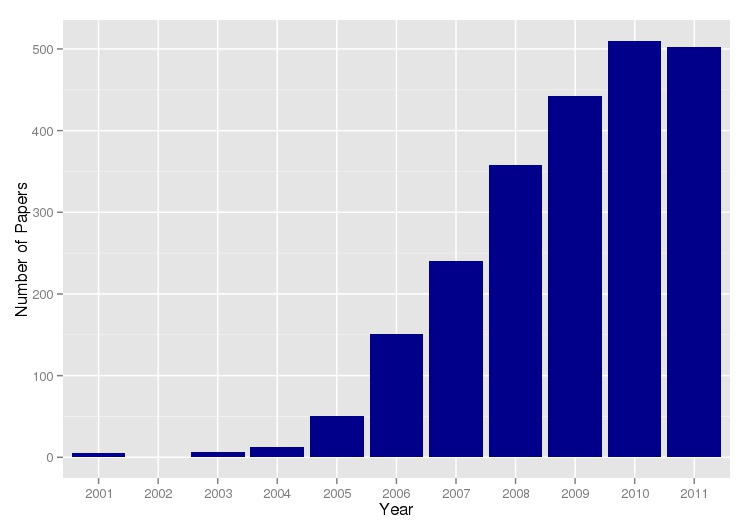
\includegraphics[width=2.4in]{figures/wp_citations_by_year.png}
%  \caption{Number of published academic articles with ``wikipedia''
%  in title by year.}
%  \label{fig:wppapers}
%  \end{centering}
%\end{wrapfigure}

\begin{wrapfigure}{r}{2.6in}
 \begin{centering}
 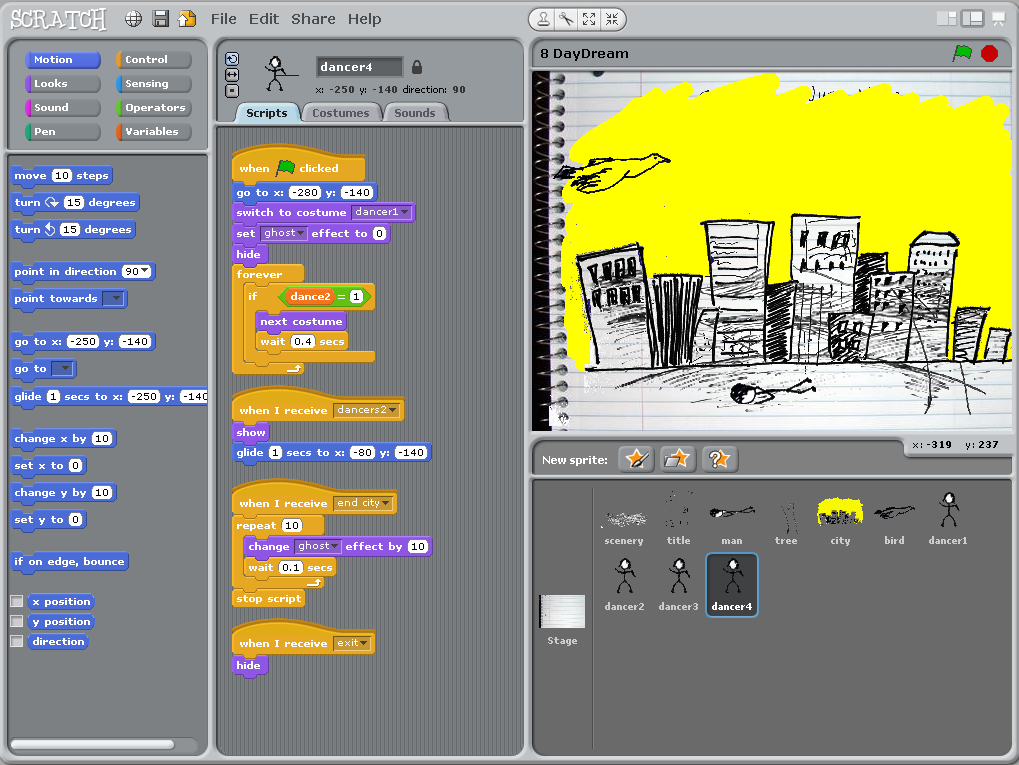
\includegraphics[width=2.6in]{figures/scratch_screenshot_default.png}
 \caption{A screenshot of the Scratch programming environment
   where users create animations and interactive games.}
 \label{fig:scratchapp}
 \end{centering}
 \vspace{-2em}
\end{wrapfigure}

In one study, I compare Wikipedia to seven attempts to create online
collaborative encyclopedia projects that were launched previously
\cite{hill_almost_2012}. Using an inductive, grounded-theory based
analysis of founder interviews and archival data, I propose four
hypotheses to explain why Wikipedia attracted many more
contributors. Although the paper's methods diverge from the
quantitative, ``big data'' approach typical of most of my work, the
research question and strategy is representative.

I have also followed this strategy in a series of quantitative studies
of the Scratch online community: a public website where millions
of users create, share, and remix interactive media. The
community is built around the Scratch programming environment: a
freely downloadable desktop application that allows amateur creators
to combine media with programming code (see Figure
\ref{fig:scratchapp}). Although Scratch is a community designed to
promote collaboration through content remixing, only about ten percent
of Scratch projects attract a second contributor.

In one study, co-authored with Andrés Monroy-Hernández and forthcoming
in American Behavioral Scientist, I test several of the most widely
cited theories associated with ``generativity'' (i.e., qualities of
technology or content that make some works more fertile ground for
collaboration). I find some support for existing theory but also find
that, across the board, factors associated with more collaboration are
also associated with less original and transformative types of
joint-work \cite{hill_remixing_2012}. In another study of Scratch
written with Monroy-Hernández and Kristina Olson, I show that this type
of superficial collaboration leads to negative reactions and community
displeasure \cite{hill_responses_2010}.

\begin{wrapfigure}{l}{2.6in}
 \vspace{-1em}
 \begin{centering}
 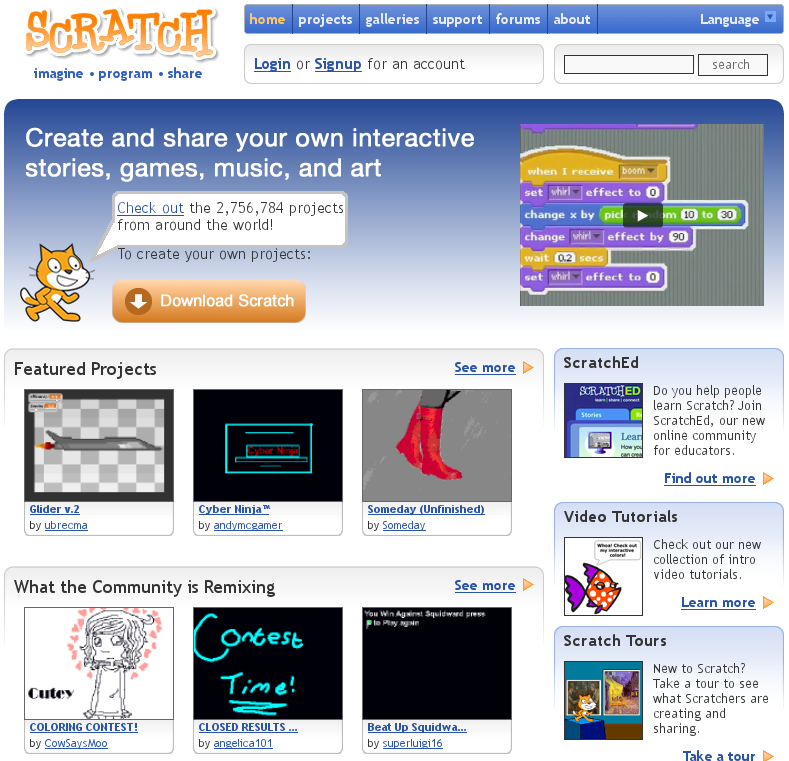
\includegraphics[width=2.6in]{figures/frontpage_modified-topremix.png}
  \caption{The front page of the Scratch online community where users
    can share and collaborate on projects.}
 \label{fig:scratchfrontpage}
 \end{centering}
 \vspace{-1.5em}
\end{wrapfigure}

This year, I am conducting a population-level analysis in a new
dataset I have created that includes 80,000 attempts at wikis (i.e.,
public, editable, websites similar to Wikipedia). In my first working
paper using this dataset, I consider inter-organizational competition
for volunteer labor and find little support for a widely cited
ecological model of collective action from sociology that treats
volunteer labor as a fixed and finite resource. Instead, I show that
contributions to different wikis on the same topic or theme are driven
primarily by environment-level changes in interest and that projects
can even benefit from complimentarities and synergies
\cite{hill_is_2012}.  By looking at failures, these studies provide
tests of several of the most influential theories of the conditions
for collective action, suggest important practical and theoretical
limitations to existing models, and point to previously untheorized
mechanisms.
\section{Reputation and Status}

Although empirical research comparing successful and unsuccessful peer
production projects has been rare, theories have been widespread. No
theory has been more influential than the suggestion that, in the
absence of pecuniary rewards, contributions to online public goods are
driven by the possibility of increased reputation and status for
contributors.

\begin{wrapfigure}{r}{0.3\textwidth}
 \vspace{-1em}
 \begin{centering}
 
\includegraphics[width=1.9in]{figures/barnstar_alone.png}
 \caption{Image of a ``barnstar'' social award given by Wikipedia
   contributors to each other to recognize positive contributions .}
 \label{fig:barnstar}
 \end{centering}
 \vspace{-1em}
\end{wrapfigure}

In a study of status-based awards in Wikipedia called ``barnstars''
(see Figure \ref{fig:barnstar}) -- a collaboration with Aaron Shaw and
Yochai Benkler -- I provide an empirical test of an influential
status-based theory of collective action from sociology. Although the
study finds support for the widely hypothesized ``virtuous cycle'' of
status rewards both causing and being caused by contributions, it also
finds that this effect is limited to a sub-population of Wikipedia
contributors -- ``signalers'' who show off their awards
\cite{hill_status_2012}. This result has broad implications for both
status-based theories of collective action as well the design of
reputation-based rewards.

In a mixed methods study of Scratch, written with a team at Microsoft
Research and nominated for best paper at the CHI 2011 conference
\cite{monroy-hernandez_computers_2011}, I present both a quantitative
analysis of a design change and in-depth interviews of users to
demonstrate how credit-giving is ineffective when it stems from an
automated system because systems fail to reinforce status-ordering
with credible human expressions of social deference and
gratitude. These studies suggest important limits to previous
theoretical work on status as a motivator for collective action, and
describe a more nuanced theoretical model.

%\newpage
\section{Design-Driven Natural Experiments}

Although nearly all of my work has important implications for the
design of socio-technical systems, I have structured much of my work
around the evaluation of technological design changes. In several
papers, I treat design changes as ``natural experiments'' that
exogenously change the ways that social structure is enacted.

\begin{wrapfigure}{r}{0.25\textwidth}
 \vspace{-1em}
 \begin{centering}
 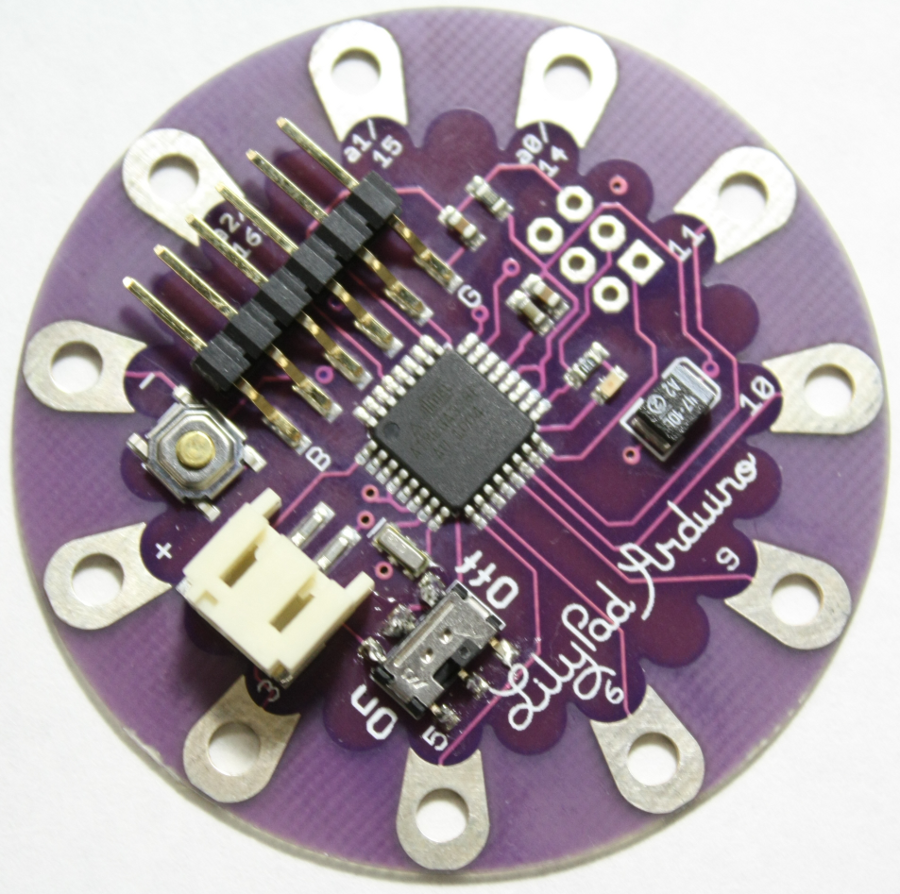
\includegraphics[width=1.5in]{figures/lilypad.png}
 \caption{A image of the LilyPad Arduino microcontroller.}
 \label{fig:lilypad}
 \end{centering}
 \vspace{-1em}
\end{wrapfigure}

For example, to evaluate the impact of status-based incentives and
collaboration in Scratch, I use a regression discontinuity framework
to measure the causal effect of increased status for collaboration
\cite{hill_causal_2012}. I show that highlighting collaborative
projects on the Scratch web page (see the bottom of Figure
\ref{fig:scratchfrontpage}) resulted in more collaboration but also
caused a decrease in the amount of total effort exerted by
contributors. Speaking to fundamental sociological work in the
literature on collective action, I present evidence that this decrease
is driven by both an the influx of new contributors and a decrease in
the effort and contributions of established participants.

In other work with Leah Buechley, I have analyzed sales records of
hobbyist microcontrollers to argue that relatively simple design
changes in the \emph{LilyPad Arduino} -- a electronics toolkit
minimally re-designed for women and girls (see Figure
\ref{fig:lilypad}) -- led to large increases in the proportion of
women contributors and drastic shifts in the type of projects created
\cite{buechley_lilypad_2010}. I have also explored how technical
errors may be able to provide similar opportunities for analysis by
interrupting normal operation of a system and revealing internal
processes that are usually hidden \cite{hill_revealing_2010}. In
addition to the important theoretical findings in these studies, this
type of work represents an important methodological advance in that it
allows for stronger causal claims while also closing the gap between
theory and design.

% or changes in socio-technical systems describing responsibility for a piece of software can lead to an important impact in the type and structure of contributions in peer production \cite{michlmayr_quality_2003}

\section{Research Agenda}

My research agenda involves further exploration of the determinants of
collection action online -- especially using a series of large new
datasets I have recently assembled. I plan to both continue on this
research trajectory and to create new social and technical
infrastructure that will allow others researchers to join me in ``big
data'' observational research with active communities. This section
outlines some future directions I plan to explore.

\emph{Understanding the Relationship Between Collective Action and
  Performance} -- My work has treated collective action and production
as ends in themselves and has largely avoided the consideration of
issues of performance, efficiency, and quality. Using my existing
datasets, I plan to compare the performance of collaborative
production to individually produced works to understand when
successful collection action leads to increased performance. For
example, in an analysis using data from Scratch which currently under
review -- done in collaboration with Monroy-Hernández -- I show
important limitations of collaboration through remixing in regards to
project quality, particularly for more artistic or media-intensive
works \cite{hill_cost_2012}.

\emph{Integrated Theory of Design for Collective Action} -- My studies
of status and reputation provide a detailed understanding of the dynamics of
collection action in relation to one set of important predictors. In future
work, I plan to evaluate the effect of governance and different
systems of authority, framing, modularity and project complexity. In
the long term, I hope to offer a broad set of principles of
design for online collection action.

\emph{Toolkits for Experimental Social Design} -- My research has been
possible through personal relationships I have with a series of
organizations with large, active, online communities (e.g., the MIT
Media Lab and the Wikimedia Foundation). These organizations, like
many others, make design changes to the software that supports their
communities to encourage contributions and improve users'
experiences. Most of the time, these organizations have very little
idea if these changes are effective. I plan to seek funding for, and
to create, a technical framework and a network of academic and
practitioner collaborators to facilitate well-designed natural
experiments by the hosts of large online communities and to share data
that allows for academic evaluation of these experiments.

Although I study cooperation, I also practice it. In graduate school,
I have collaborated with a large group of co-authors in many academic
departments. I intend to continue doing so. In sum, my research uses
design to contribute to social scientific theories of collective
action, and uses theories of collective action to influence
design. Although my research settings are online communities, I
believe my work has implications for a broad range of disciplines and
fields.

% bibliography here
\renewcommand{\bibsection}{\section{\bibname}\prebibhook}
\baselineskip 14.2pt
\bibliography{refs-processed}
\bibliographystyle{unsrt}

\end{document}

